\section[Performance of the charged particle tracking system (Simon)]{Performance of the charged particle tracking system}
\subsection{Track reconstruction}

The first stage in track reconstruction is pattern recognition.  Hits in adjacent
 layers in the FDC in each package are formed into track segments that are 
linked together with other segments in other packages to form FDC track 
candidates using a helical model for the track parameters.
Hits in adjacent rings in the axial layers of the CDC are also associated into 
segments that are linked together with other segments in other axial layers
and fitted with circles in the projection perpendicular to the beam line. We 
then find intersections between these circles and the stereo wires and perform 
a linear fit to find a z-position near the beam line and the tangent to the dip
 angle $\lambda=\pi/2-\theta$.  These parameters in addition to the circle fit 
parameters form a CDC track candidate for each set of linked axial and stereo 
layers.   We link FDC and CDC track candidates together that emerge from the 
target in the $\theta=5^\circ-20^\circ$ range that pass through both the FDC 
and the CDC.

The second stage uses a Kalman Filter \cite{KalmanFilter, KalmanFilter2} to find the fitted track parameters
\{z,D,$\phi$,$\tan\lambda$,$q/p_T$\}
at the position of closest approach of the track to the beam line using the 
track candidate parameters as an initial guess.  Here $D$ is the signed 
distance of closest approach to the beam line.  The Kalman Filter proceeds in 
steps from
the hits farthest from the beam line toward the beam line, taking into account
energy loss and multiple scattering at each step along the way and incorporating
a map of the magnetic field within the bore of the solenoid magnet.  For the 
first 
initial pass of the filter we do not use the drift time information from the 
wires.  We assume that each particle is a pion, except for low momentum track 
candidates (p$<$0.8 GeV/c), for which we redo the fits with a proton hypothesis.

At the beginning of the third stage we match each fitted track from the second 
stage to the start counter, the time-of-flight scintillators, the BCAL and the 
FCAL to determine a start time $t_0$ so that the drift time to each wire 
associated with the track can be used in the fit.  Each track is refitted with
the drift information multiple times using the set \{$e^\pm,\pi^\pm,K^\pm,p^\pm$\} 
of mass hypotheses.




\subsection{Momentum resolution}

The momentum resolution as a function of angle and magnitude for pions and 
protons is shown in Fig.~\ref{fig:dp_p}.  The angular resolution is shown in 
Fig.~\ref{fig:angle res}.


\begin{figure}[tbp]
\begin{center}
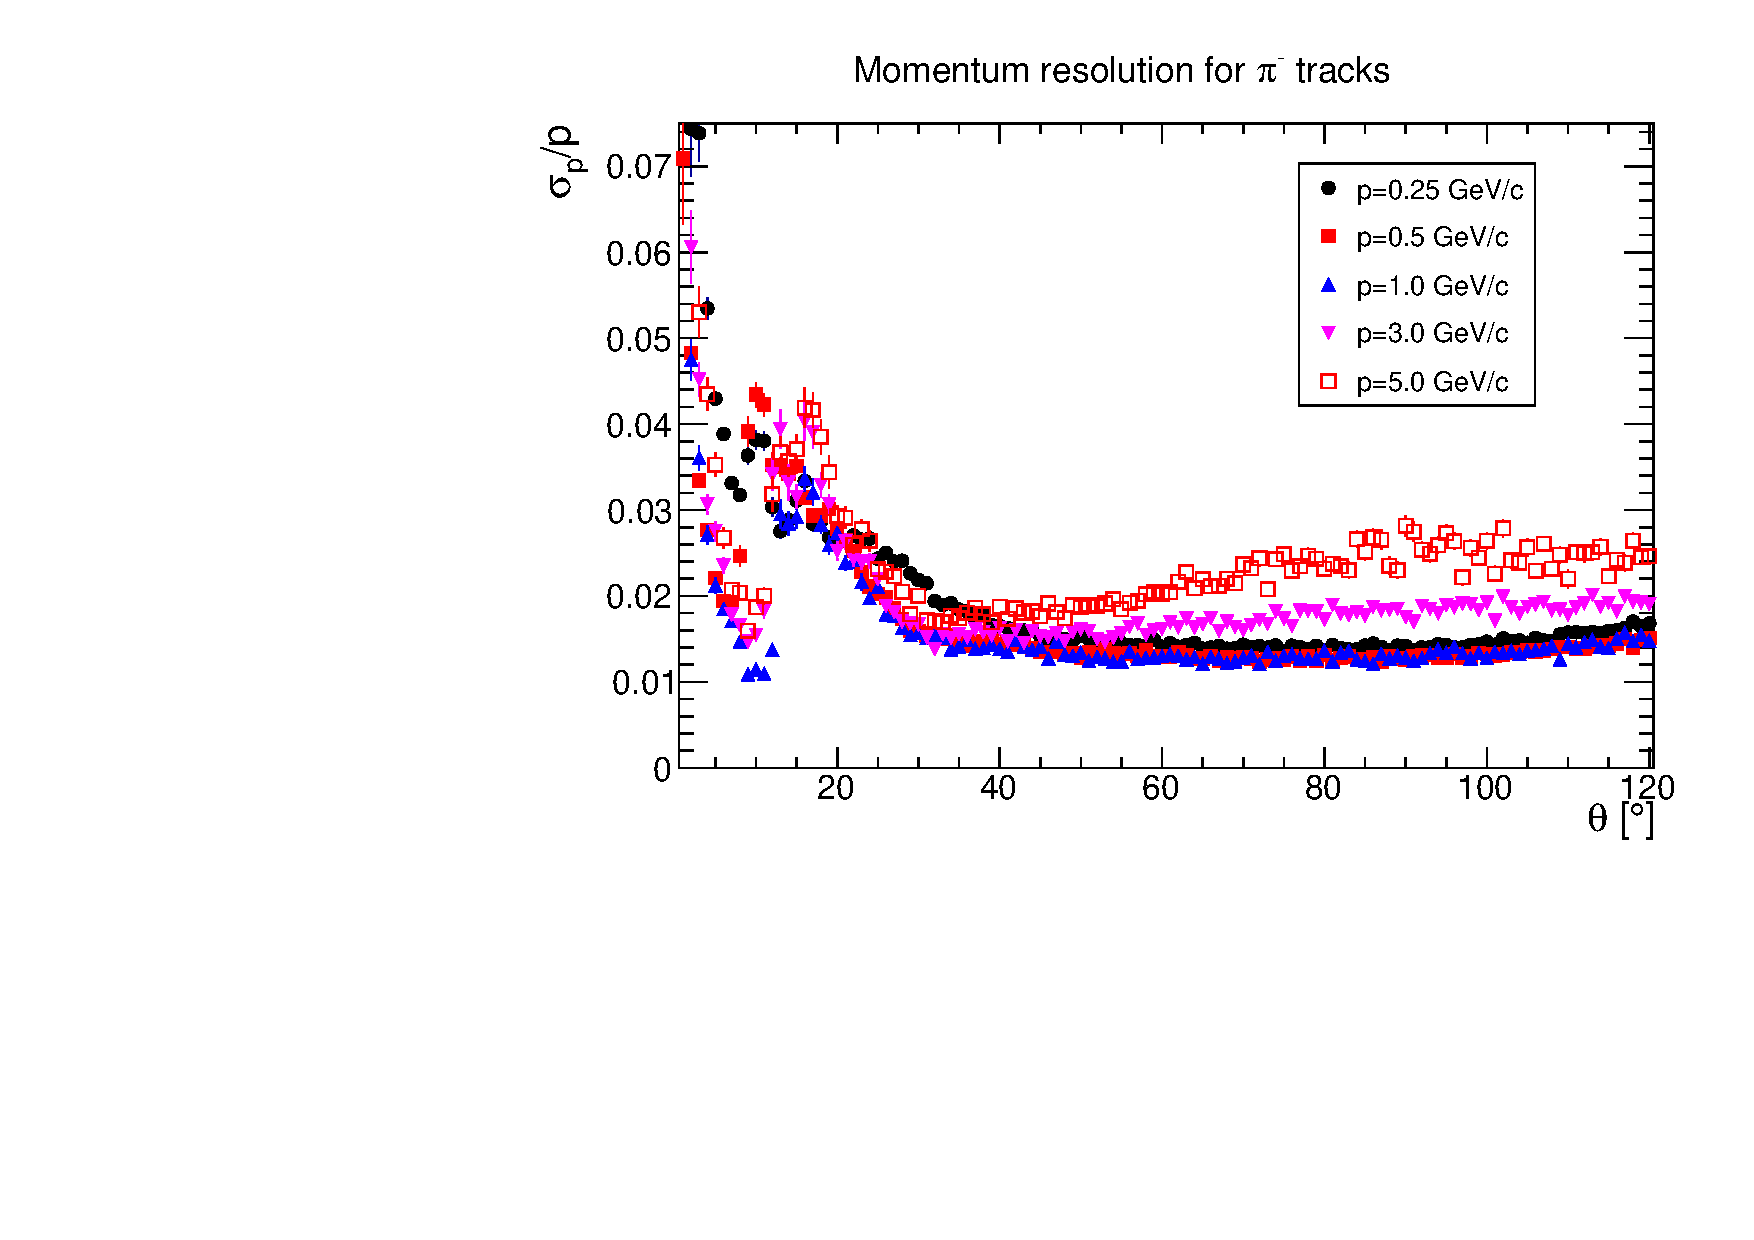
\includegraphics[width=0.45\textwidth]{figures/PionMomentumResolution.pdf}
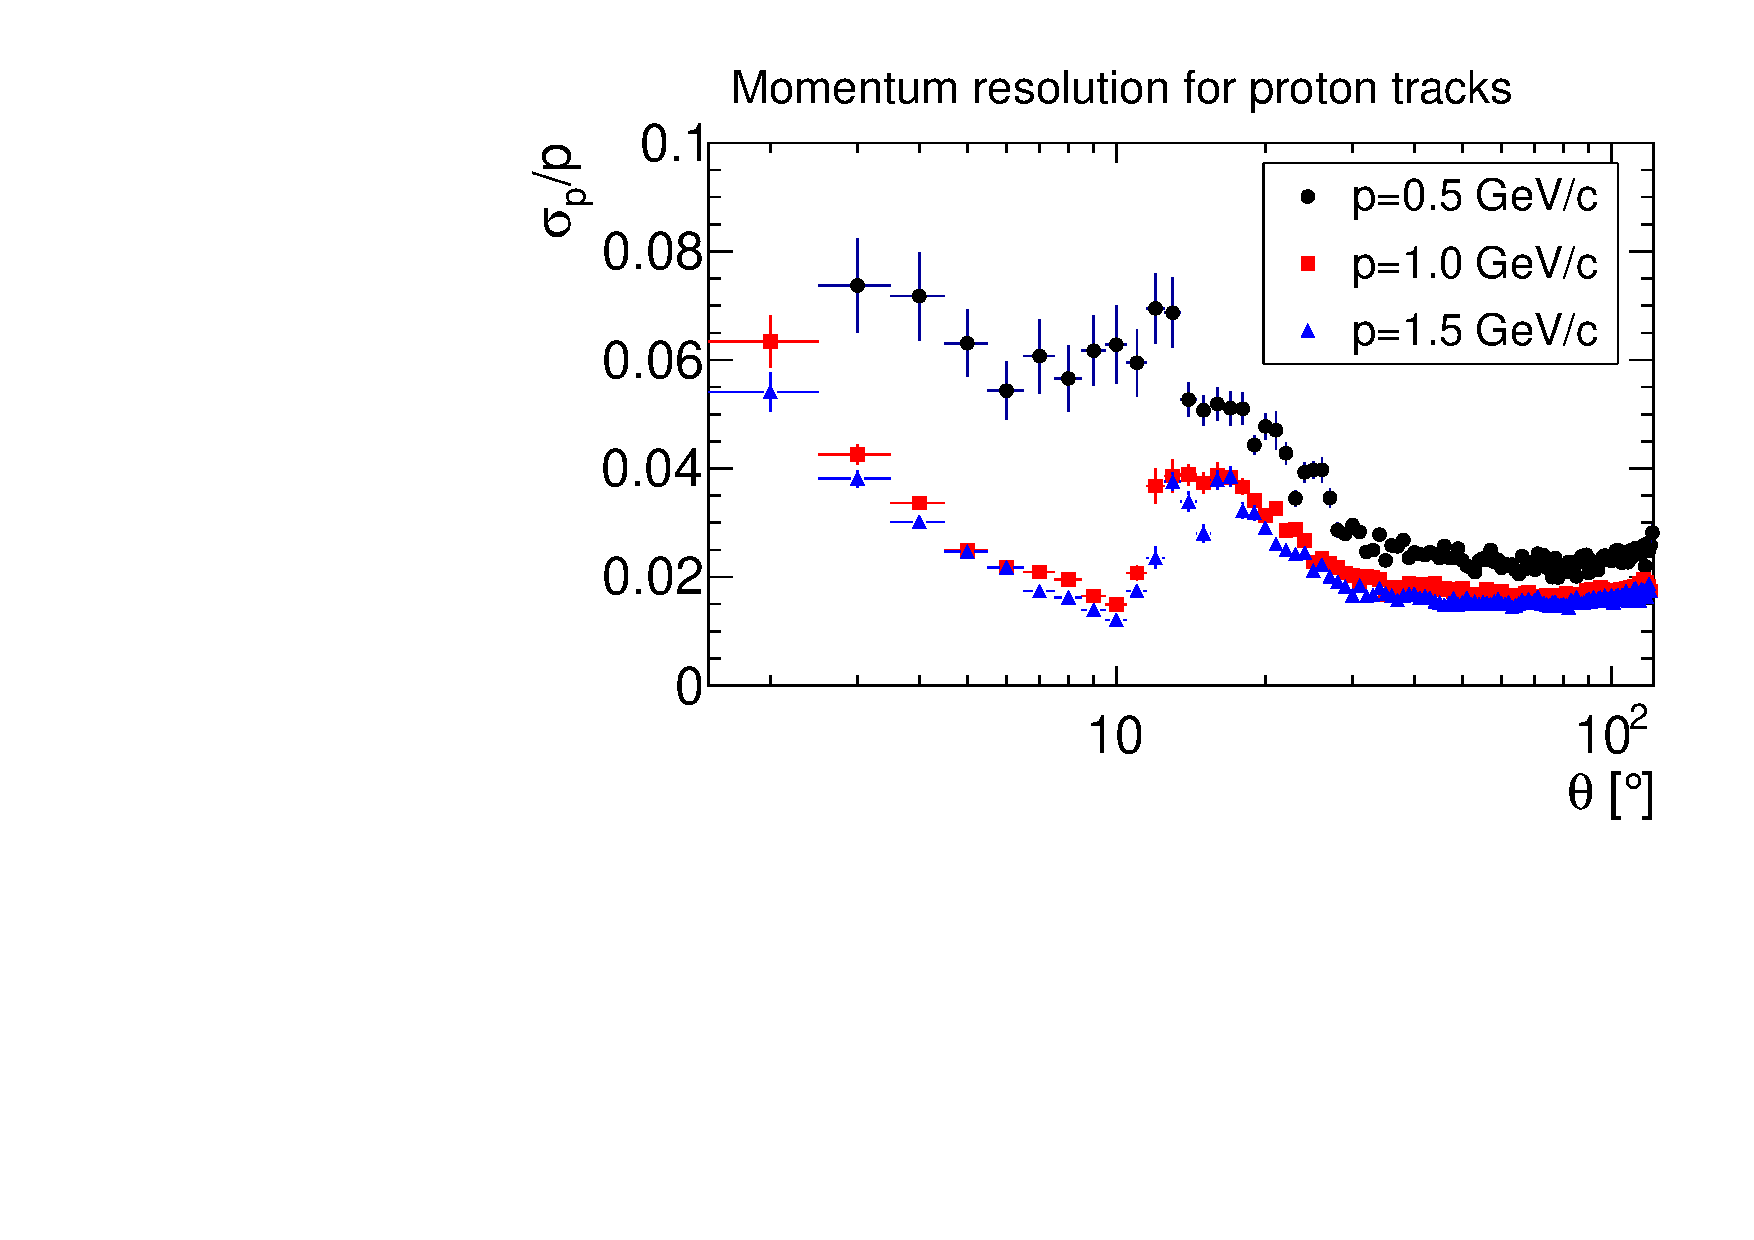
\includegraphics[width=0.45\textwidth]{figures/ProtonMomentumResolution.pdf}
\caption{\label{fig:dp_p} (Left) Momentum resolution for $\pi^-$ tracks.
(Right) Momentum resolution for proton tracks. (Color online)}
\end{center}
\end{figure}

\begin{figure}[tbp]
\begin{center}
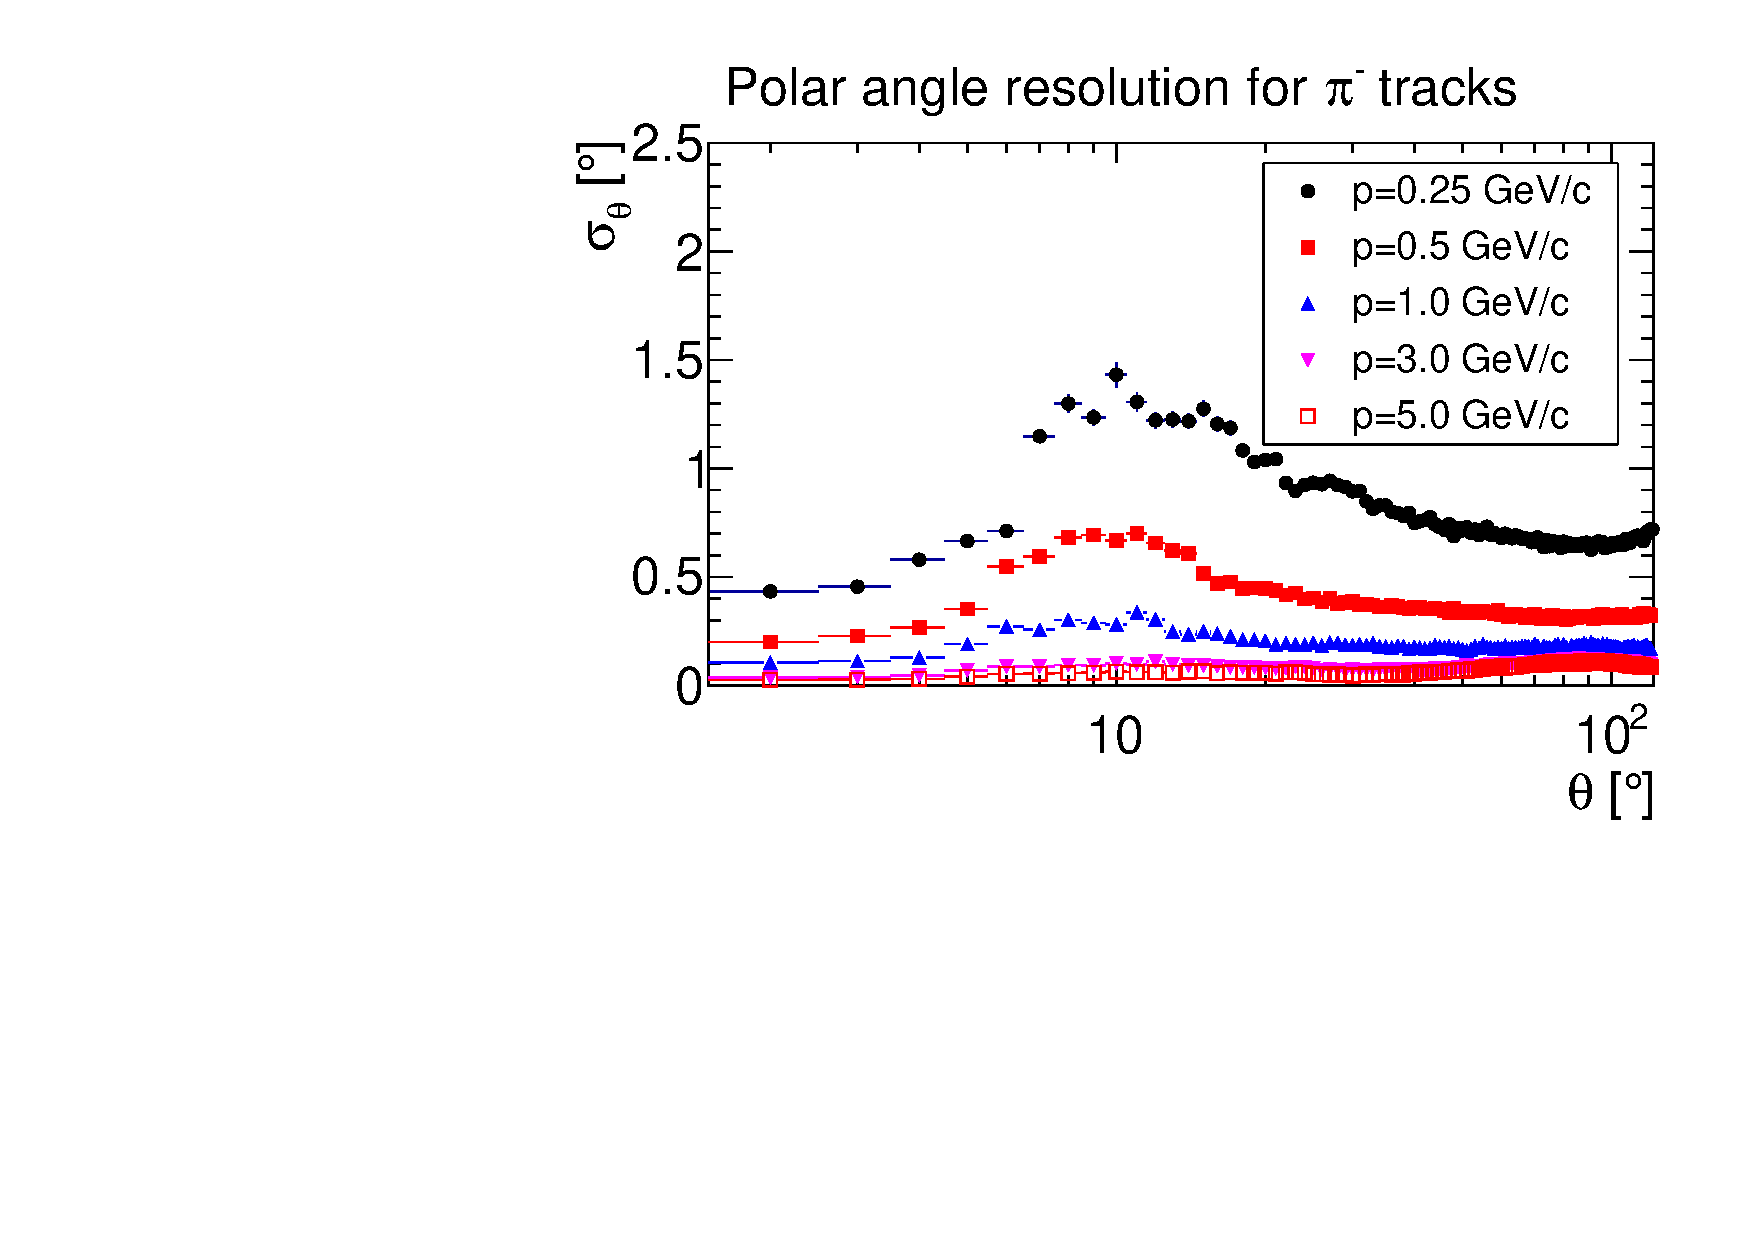
\includegraphics[width=0.45\textwidth]{figures/PionThetaResolution.pdf}
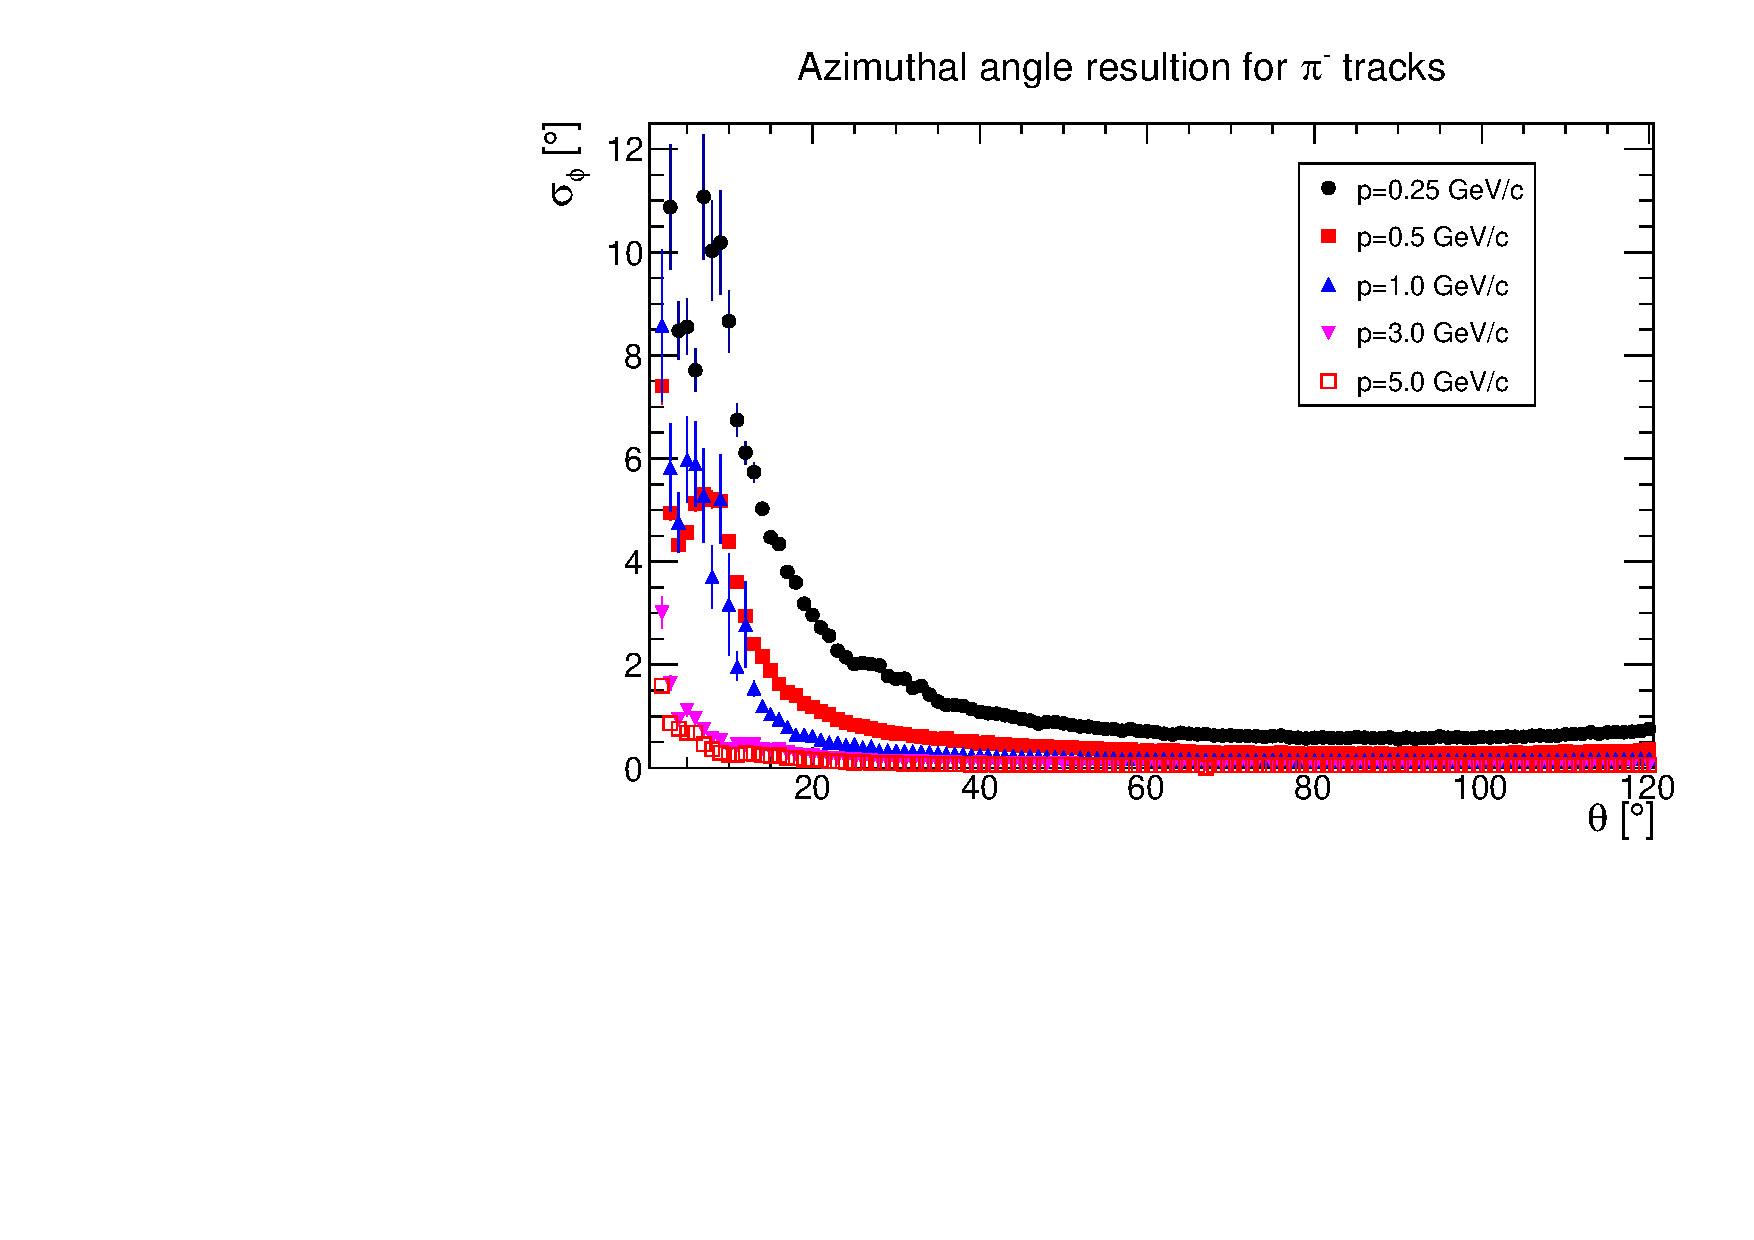
\includegraphics[width=0.45\textwidth]{figures/PionPhiResolution.pdf}
\caption{\label{fig:angle res} (Left) Polar angle resolution for $\pi^-$ tracks.
(Right) Azimuthal angle resolution for $\pi^-$ tracks.
 (Color online)}
\end{center}
\end{figure}


\subsection{Vertex resolution}

The thin windows of the cryogenic target and the exit window of the target
vacuum chamber provide a means to estimate the 
vertex resolution of the tracking system.  We use pairs of tracks from 
``empty target'' runs to reconstruct these windows as illustrated in 
Fig.~\ref{fig:z-vertex}.  We required $d<1$ cm, where $d$ is the 
distance-of-closest-approach between the two tracks. The ``vertex'' position 
is at the mid-point of the line segment of length $d$ connecting the two tracks.
The estimated z-position resolution is 3 mm.

\begin{figure}[tbp]
\begin{center}
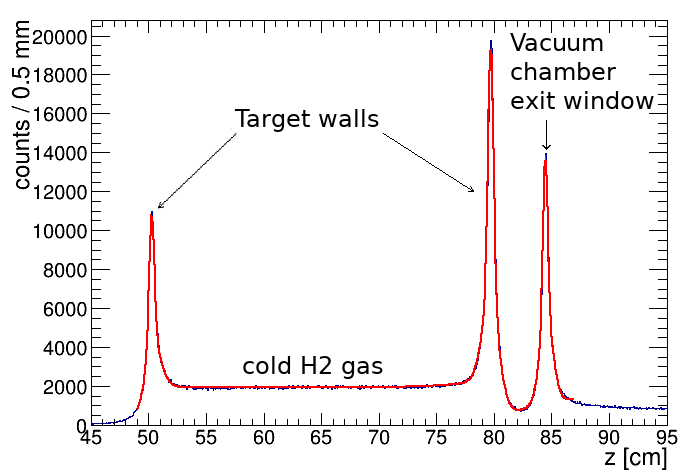
\includegraphics[width=0.7\textwidth]{figures/zvertex.png}  
\caption{\label{fig:z-vertex} Reconstructed vertex positions within 1 cm radial
 distance with respect to the beam line for an empty target run.  The curve shows the result of a fit to the vertex distribution used to determine the vertex
resolution.  (Color online). 
}   
\end{center}  
\end{figure}

